% !TEX root = ../main.tex
\chapter{Ceros, conteo y atracción}\label{sec:ceros_acotacion}

El Capítulo~\ref{sec:matricial} dejó fijada la capa macroscópica del problema: el umbral singular en el índice $m$ detecta cuándo la inestabilidad del operador de multiplicación queda confinada a un número finito de direcciones. En este capítulo damos el paso final y traducimos esa información al lenguaje de los ceros de los polinomios ortogonales de Sobolev.

La lectura correcta tiene dos niveles. Primero aparece un puente macroscópico: los ceros se leen como autovalores de $\mathbf D_n^t$ y la desigualdad de Weyl--Horn convierte el umbral singular en un techo de conteo. Después entra la capa fina: la reducción racional exterior de $\pi_{n+1}(z)/z^{n+1}$ y el Teorema de Rouché identifican dónde caen realmente esos ceros y qué perfil adoptan en cada régimen geométrico. Esa separación será esencial a lo largo de todo el capítulo.

\section{Autovalores, umbral singular y Weyl--Horn}\label{sec:weyl_horn}

Antes de distinguir regímenes, fijamos el mecanismo común que solo da control macroscópico. El problema de los ceros ya quedó traducido al lenguaje matricial en el Capítulo~\ref{sec:matricial}. En la Proposición~\ref{prop:charpoly_truncada} vimos que la matriz de Hessenberg truncada $\mathbf D_n$ codifica la acción de multiplicar por $z$ sobre $\mathbb P_n=[\phi_0,\dots,\phi_n]$, y que su polinomio característico reproduce, salvo normalización, al polinomio ortogonal siguiente.

\begin{prop}\label{prop:autovalores_ceros}
	Para cada $n \ge 0$, los ceros del polinomio ortonormal $\phi_{n+1}(z)$ coinciden, contando multiplicidades, con los autovalores de la sección transpuesta $\mathbf{D}_n^t$:
	\[
		\sigma(\mathbf{D}_n^t) = \{z \in \mathbb{C} : \phi_{n+1}(z) = 0\}.
	\]
\end{prop}

\begin{proof}
	La matriz $\mathbf{D}_n$ representa la compresión del operador de multiplicación $\D$ al subespacio $\mathbb P_n$ en la base $\{\phi_k\}_{k=0}^n$. Como la multiplicación por $z$ aumenta el grado en una unidad, $\mathbf{D}_n$ tiene estructura de Hessenberg superior: sus entradas satisfacen $d_{ij}=0$ para $i>j+1$. Esto implica que para cualquier $\lambda\in\C$,
	\[
		\det(\lambda I_{n+1}-\mathbf{D}_n^t)=\det(\lambda I_{n+1}-\mathbf{D}_n)
		=\phi_{n+1}(\lambda)/\gamma_{n+1},
	\]
	donde $\gamma_{n+1}$ es el coeficiente director de $\phi_{n+1}$. La última igualdad es la identidad característica estándar para matrices de Hessenberg asociadas a polinomios ortogonales (véase \cite{szego1975orthogonal}, §3.1, o \cite{gohberg1969introduction}, Cap.~VI). Por tanto, $\lambda$ es autovalor de $\mathbf{D}_n^t$ si y solo si $\phi_{n+1}(\lambda)=0$.
\end{proof}

\begin{defn}\label{def:radio_espectral}
	El \emph{radio espectral} de una matriz cuadrada $A \in \mathcal{M}_n(\mathbb{C})$, denotado $\rho(A)$, se define como $\rho(A)=\max\{|\lambda| : \lambda \in \sigma(A)\}$.
\end{defn}

Aplicado a $A=\mathbf D_n^t$, este radio espectral mide directamente el módulo del cero más exterior de $\phi_{n+1}$. Además, para toda matriz se tiene $\rho(A)\le \|A\|_2=\sigma_0(A)$, de modo que $\rho(\mathbf D_n^t)\le \sigma_{0,n}$.
Esto da un control grosero del tamaño de los ceros. El siguiente paso macroscópico consiste en mirar no un solo autovalor, sino el producto de los $k$ autovalores de mayor módulo.

\begin{lem}\label{lem:weyl_horn}
	Sea $A\in\mathcal{M}_{n+1}(\mathbb{C})$ con autovalores $\lambda_0,\dots,\lambda_n$
	ordenados por módulo decreciente y valores singulares
	$\sigma_0\ge\sigma_1\ge\cdots\ge\sigma_n\ge 0$. Entonces
	\[
		\prod_{j=0}^{k-1}|\lambda_j|\;\le\;\prod_{j=0}^{k-1}\sigma_j,
		\qquad k=1,\dots,n+1,
	\]
	con igualdad para $k=n+1$.
\end{lem}

\begin{proof}
	Véase la demostración en \cite[Sec.~3.3]{horn2012matrix}.
\end{proof}

La desigualdad anterior muestra que el producto de los $k$ autovalores de mayor módulo no puede superar el producto de los $k$ valores singulares mayores. Por tanto, una vez fijado el umbral singular, el escape espectral queda restringido. En el régimen puramente exterior, $\sigma_{j,n}\to +\infty$ para $j<m$ y $\lim_{n\to\infty}\sigma_{m,n}\le R$; en el caso mixto al menos se conserva la cota abstracta $\lim_{n\to\infty}\sigma_{m,n}\le Q_m(\D)<\infty$.
En consecuencia, a partir del índice $m$ el escape de autovalores deja de comportarse como en un régimen completamente inestable. Este control sigue siendo solo macroscópico: acota cuántos ceros pueden quedar en $|z|>R+\varepsilon$, pero no decide todavía junto a qué átomos aparecen ni qué escala local rige en frontera. Para eso hará falta pasar a la reducción racional exterior y a Rouché.

\section{Conteo exacto en el régimen puramente exterior}\label{sec:conteo_ceros}

En esta sección, \emph{puramente exterior} significa estrictamente exterior, es decir, $|c_k|>R$ para todo $k=1,\dots,m$. Los posibles puntos de frontera, caracterizados por $|c_k|=R$ para algún $k\le m$, se tratarán por separado más adelante. El Lema~\ref{lem:weyl_horn} solo da un techo: a lo sumo hay $m$ ceros exteriores. El objetivo ahora es convertir ese techo en un conteo exacto mediante la reducción racional exterior de $\pi_{n+1}(z)/z^{n+1}$ y el Teorema de Rouché.

Al normalizar los polinomios mónicos de Sobolev, este cociente converge a una función racional $F(z)$ con un cero en cada átomo exterior y polos en el interior del disco. Esa es la pieza que convierte el techo macroscópico en conteo exacto.

\begin{lem}\label{lem:sumas_geometricas_ponderadas}
	Para $\xi\in\mathbb C\setminus\{1\}$ y $n\ge1$ definimos
	\[
		S_n(\xi):=\sum_{j=1}^n j\xi^{j-1},
		\qquad
		T_n(\xi):=\sum_{j=1}^n j^2\xi^{j-1}.
	\]
	Entonces
	\[
		S_n(\xi)=\frac{1-(n+1)\xi^n+n\xi^{n+1}}{(1-\xi)^2}
	\]
	y
	\[
		T_n(\xi)=\frac{1+\xi-(n+1)^2\xi^n+(2n^2+2n-1)\xi^{n+1}-n^2\xi^{n+2}}{(1-\xi)^3}.
	\]
	En particular, para todo compacto $K\subset\{\xi\in\mathbb C:|\xi|>1\}$,
	\[
		\frac{S_n(\xi)}{n\xi^n}\longrightarrow \frac{1}{\xi-1},
		\qquad
		\frac{T_n(\xi)}{n^2\xi^n}\longrightarrow \frac{1}{\xi-1}
	\]
	uniformemente en $K$.
\end{lem}

\begin{proof}
	Las identidades cerradas se obtienen derivando las sumas geométricas finitas
	\[
		\sum_{j=0}^n \xi^j=\frac{1-\xi^{n+1}}{1-\xi}
	\]
	y multiplicando luego por $\xi$ cuando corresponde. Si $|\xi|>1$, en las fórmulas anteriores los términos dominantes son $n\xi^{n+1}$ en $S_n$ y $-n^2\xi^{n+2}$ en $T_n$, de donde se siguen las dos convergencias. La uniformidad en compactos de $\{|\xi|>1\}$ es inmediata porque los denominadores $(\xi-1)$ quedan uniformemente separados de cero.
\end{proof}

\begin{lem}\label{lem:cotas_sumas_geometricas_ponderadas}
	Sea $K\subset\C$ compacto. Entonces existe una constante $C_K>0$ tal que, para todo $n\ge1$ y todo $\xi\in K$,
	\[
		|S_n(\xi)|\le C_K\,n^2\,\max\{1,|\xi|\}^n,
		\qquad
		|T_n(\xi)|\le C_K\,n^3\,\max\{1,|\xi|\}^n.
	\]
\end{lem}

\begin{proof}
	Sea $M:=\max\{1,\sup_{\xi\in K}|\xi|\}$. Para todo $\xi\in K$,
	\[
		|S_n(\xi)|\le \sum_{j=1}^n j|\xi|^{j-1}
		\le \sum_{j=1}^n jM^{j-1}
		\le n^2 M^n,
	\]
	y análogamente
	\[
		|T_n(\xi)|\le \sum_{j=1}^n j^2|\xi|^{j-1}
		\le \sum_{j=1}^n j^2M^{j-1}
		\le n^3 M^n.
	\]
	Absorbiendo las constantes numéricas en $C_K$ se obtienen las cotas uniformes anunciadas.
\end{proof}

\begin{lem}\label{lem:modelo_un_atomo_exterior}
	Sea
	\[
		\langle p,q\rangle_S
		=
		\int_{\mathbb S_R}p(z)\overline{q(z)}\,d\mathbf m_{0;R}(z)
		+
		p'(c)\overline{q'(c)},
		\qquad |c|>R,
	\]
	y sea $\pi_{n+1}$ el polinomio mónico ortogonal de Sobolev de grado $n+1$.
	Entonces
	\[
		\pi_{n+1}(z)=z^{n+1}-\alpha_n\sum_{j=1}^n j\frac{\overline c^{\,j-1}}{R^{2j}}z^j,
	\]
	donde
	\[
		\alpha_n=
		\frac{(n+1)c^n}{1+\dfrac1{R^2}\sum_{j=1}^n j^2\left(\dfrac{|c|^2}{R^2}\right)^{j-1}}.
	\]
	Además,
	\[
		\frac{\pi_{n+1}(z)}{z^{n+1}}
		\xrightarrow[n\to\infty]{}
		\frac{\overline c\,(z-c)}{\overline c z-R^2}
	\]
	uniformemente en compactos de $\{z\in\mathbb C:|z|>R\}$. En consecuencia, para todo $\varepsilon>0$ suficientemente pequeño, $\pi_{n+1}$ tiene, para $n$ suficientemente grande, exactamente un cero en $\overline{\mathbb D_\varepsilon(c)}$, y ese cero converge a $c$.
\end{lem}

\begin{proof}
	Escribimos
	\[
		\pi_{n+1}(z)=z^{n+1}+\sum_{j=0}^n a_{j,n}z^j.
	\]
	La ortogonalidad frente a $1$ da $a_{0,n}=0$, porque la parte derivativa de $1$ es nula y $z^{n+1}$ es ortogonal a las constantes en $L^2(\mathbf m_{0;R})$.

	Para $1\le k\le n$, la ortogonalidad frente a $z^k$ da
	\[
		0=\langle \pi_{n+1},z^k\rangle_S
		=a_{k,n}R^{2k}+\pi_{n+1}'(c)\,k\overline c^{\,k-1},
	\]
	de donde
	\[
		a_{k,n}=-\pi_{n+1}'(c)\,k\frac{\overline c^{\,k-1}}{R^{2k}}.
	\]
	Sustituyendo en la identidad para la derivada en $c$ se obtiene
	\begin{align*}
		\pi_{n+1}'(c)
		 & =(n+1)c^n+\sum_{j=1}^n j a_{j,n}c^{j-1} \\
		 & =(n+1)c^n-\pi_{n+1}'(c)\,\frac1{R^2}
		\sum_{j=1}^n j^2\left(\frac{|c|^2}{R^2}\right)^{j-1},
	\end{align*}
	y por tanto $\pi_{n+1}'(c)=\alpha_n$. Esto prueba la fórmula exacta.

	Sea ahora $t=\frac{\overline c z}{R^2}$.
	Como $|c|>R$ y trabajamos sobre compactos contenidos en $\{|z|>R\}$, se tiene $|t|>1$ uniformemente. La expresión anterior puede reescribirse como
	\[
		\frac{\pi_{n+1}(z)}{z^{n+1}}
		=
		1-
		\frac{n\overline c^{\,n}\alpha_n}{R^{2n}}
		\frac{1}{R^2}
		\frac{S_n(t)}{nt^n}.
	\]
	Por el Lema~\ref{lem:sumas_geometricas_ponderadas},
	\[
		\frac{n\overline c^{\,n}\alpha_n}{R^{2n}}
		\longrightarrow |c|^2-R^2,
		\qquad
		\frac{1}{R^2}\frac{S_n(t)}{nt^n}\longrightarrow \frac{1}{\overline c z-R^2},
	\]
	uniformemente en compactos de $\{|z|>R\}$. En consecuencia,
	\[
		\frac{\pi_{n+1}(z)}{z^{n+1}}
		\longrightarrow
		1-\frac{|c|^2-R^2}{\overline c z-R^2}
		=
		\frac{\overline c z-|c|^2}{\overline c z-R^2}
		=
		\frac{\overline c\,(z-c)}{\overline c z-R^2}.
	\]

	Tomemos ahora $\varepsilon>0$ con $\overline{\mathbb D_\varepsilon(c)}\subset\{|z|>R\}$. El límite tiene un cero simple en $c$ y no se anula sobre $\partial\mathbb D_\varepsilon(c)$. Por convergencia uniforme, para $n$ grande las funciones $\pi_{n+1}(z)/z^{n+1}$ y $\overline c(z-c)/(\overline c z-R^2)$ tienen el mismo número de ceros en $\mathbb D_\varepsilon(c)$; por el teorema de Rouché, ese número es $1$.

	Además, el Lema~\ref{lem:conteo_exterior_reciproco} aplicado con $m=1$ muestra que, para todo $\eta\in(0,|c|-R)$, existe exactamente un cero de $\pi_{n+1}$ en $|z|>R+\eta$ cuando $n$ es grande. Ese cero es precisamente el localizado en $\mathbb D_\varepsilon(c)$, luego converge a $c$. Por tanto, el atractor del modelo de un átomo es el propio átomo $c$.
\end{proof}

\begin{lem}\label{lem:sistema_finito_atraccion}
	Sea
	\[
		\langle p,q\rangle_S
		=
		\int_{\mathbb S_R}p(z)\overline{q(z)}\,d\mathbf m_{0;R}(z)
		+
		\sum_{\ell=1}^m p'(c_\ell)\overline{q'(c_\ell)},
		\qquad |c_\ell|>R,
	\]
	con $c_1,\dots,c_m$ distintos, y sea $\pi_{n+1}(z)=z^{n+1}+\sum_{j=0}^n a_{j,n}z^j$ el polinomio mónico ortogonal de Sobolev.
	Definiendo $v_{\ell,n}:=\pi_{n+1}'(c_\ell)$ para $1\le \ell\le m$,
	se tiene $a_{0,n}=0$ y, para $1\le j\le n$,
	\[
		a_{j,n}=-jR^{-2j}\sum_{\ell=1}^m v_{\ell,n}\overline c_\ell^{\,j-1}.
	\]
	Además, el vector $v_n=(v_{1,n},\dots,v_{m,n})^t$ satisface el sistema lineal
	\[
		\sum_{\ell=1}^m
		\left[
			\delta_{r\ell}+
			\frac1{R^2}T_n\!\left(\frac{c_r\overline c_\ell}{R^2}\right)
			\right]v_{\ell,n}
		=(n+1)c_r^n,
		\qquad 1\le r\le m.
	\]
\end{lem}

\begin{proof}
	La ortogonalidad frente a $1$ da, de nuevo, $a_{0,n}=0$. Para $1\le k\le n$,
	\[
		0=\langle \pi_{n+1},z^k\rangle_S
		=a_{k,n}R^{2k}+k\sum_{\ell=1}^m v_{\ell,n}\overline c_\ell^{\,k-1},
	\]
	y por tanto
	\[
		a_{k,n}=-kR^{-2k}\sum_{\ell=1}^m v_{\ell,n}\overline c_\ell^{\,k-1}.
	\]
	Derivando y evaluando en $c_r$ obtenemos
	\begin{align*}
		v_{r,n}
		 & =(n+1)c_r^n+\sum_{j=1}^n ja_{j,n}c_r^{j-1} \\
		 & =(n+1)c_r^n-
		\frac1{R^2}
		\sum_{\ell=1}^m v_{\ell,n}
		\sum_{j=1}^n j^2\left(\frac{c_r\overline c_\ell}{R^2}\right)^{j-1},
	\end{align*}
	que es exactamente el sistema anunciado.
\end{proof}

\begin{lem}\label{lem:conteo_exterior_reciproco}
	Sea
	\[
		\langle p,q\rangle_S
		=
		\int_{\mathbb S_R}p(z)\overline{q(z)}\,d\mathbf m_{0;R}(z)
		+
		\sum_{k=1}^m p'(c_k)\overline{q'(c_k)},
	\]
	donde $c_1,\dots,c_m$ son distintos y satisfacen $|c_k|>R$ para todo $k$. Sea $\pi_{n+1}$ el polinomio mónico ortogonal de Sobolev de grado $n+1$. Fijado
	\[
		0<\varepsilon<\min_{1\le k\le m}(|c_k|-R),
	\]
	se tiene
	\[
		\frac{\pi_{n+1}(z)}{z^{n+1}}
		\longrightarrow
		F(z):=\prod_{k=1}^m\frac{z-c_k}{z-R^2/\overline c_k}
	\]
	uniformemente sobre $|z|=R+\varepsilon$; de hecho, la convergencia es uniforme en compactos de $\{|z|>R+\varepsilon\}$. En particular, para $n$ suficientemente grande, $\pi_{n+1}$ tiene exactamente $m$ ceros en $\{|z|>R+\varepsilon\}$.
\end{lem}

\begin{proof}
	Sea $C=(C_{r\ell})_{1\le r,\ell\le m}$, con $C_{r\ell}:=\frac{1}{c_r\overline c_\ell-R^2}$.
	Esta es una matriz de Cauchy con parámetros $x_r=c_r$ y $y_\ell=-R^2/\overline c_\ell$. Como los $c_r$ son distintos y también lo son los $R^2/\overline c_\ell$, se tiene $x_r-y_\ell\neq0$ para todo par $(r,\ell)$ y el determinante de Cauchy es no nulo; luego $C$ es invertible.

	Definimos $\beta_n:=\bigl(\beta_{1,n},\dots,\beta_{m,n}\bigr)^t$, donde $\beta_{\ell,n}:=\frac{n\overline c_\ell^{\,n}}{R^{2n}}v_{\ell,n}$.
	Dividiendo el sistema del Lema~\ref{lem:sistema_finito_atraccion} por $nc_r^n$ obtenemos
	\[
		C_n\beta_n=\left(1+\frac1n\right)\mathbf 1,
	\]
	donde $\mathbf 1=(1,\dots,1)^t$ y
	\[
		(C_n)_{r\ell}
		=
		\delta_{r\ell}\frac{R^{2n}}{n^2|c_r|^{2n}}
		+
		\frac{1}{n^2R^2}
		\frac{T_n\!\left(\dfrac{c_r\overline c_\ell}{R^2}\right)}{\left(\dfrac{c_r\overline c_\ell}{R^2}\right)^n}.
	\]
	Puesto que $\bigl|c_r\overline c_\ell/R^2\bigr|>1$, el Lema~\ref{lem:sumas_geometricas_ponderadas} da
	\[
		(C_n)_{r\ell}\longrightarrow \frac{1}{c_r\overline c_\ell-R^2}=C_{r\ell}.
	\]
	Por invertibilidad de $C$, también $C_n$ es invertible para $n$ grande y
	\[
		\beta_n\longrightarrow \beta:=C^{-1}\mathbf 1.
	\]

	Ahora usamos la fórmula exacta de los coeficientes:
	\[
		\frac{\pi_{n+1}(z)}{z^{n+1}}
		=
		1-
		\sum_{\ell=1}^m
		\beta_{\ell,n}
		\frac{1}{R^2}
		\frac{S_n\!\left(\dfrac{\overline c_\ell z}{R^2}\right)}{n\left(\dfrac{\overline c_\ell z}{R^2}\right)^n}.
	\]
	Si $K\subset\{|z|>R+\varepsilon\}$ es compacto, entonces $\bigl|\overline c_\ell z/R^2\bigr|>1$ uniformemente en $K$; por el Lema~\ref{lem:sumas_geometricas_ponderadas},
	\[
		\frac{1}{R^2}
		\frac{S_n\!\left(\dfrac{\overline c_\ell z}{R^2}\right)}{n\left(\dfrac{\overline c_\ell z}{R^2}\right)^n}
		\longrightarrow
		\frac{1}{\overline c_\ell z-R^2}
	\]
	uniformemente en $K$. Concluimos que
	\[
		\frac{\pi_{n+1}(z)}{z^{n+1}}
		\longrightarrow
		1-\sum_{\ell=1}^m\frac{\beta_\ell}{\overline c_\ell z-R^2}
	\]
	uniformemente en compactos de $\{|z|>R+\varepsilon\}$.

	Además, para cada $r$,
	\[
		1-\sum_{\ell=1}^m\frac{\beta_\ell}{c_r\overline c_\ell-R^2}=0,
	\]
	porque $C\beta=\mathbf 1$. Como la función límite vale $1$ en infinito y todos sus polos $R^2/\overline c_\ell$ están dentro de $\mathbb D_R$, la unicidad de la descomposición racional implica que
	\[
		F(z)=\prod_{\ell=1}^m\frac{z-c_\ell}{z-R^2/\overline c_\ell}.
	\]

	Pasamos ahora a la variable recíproca $w=1/z$ y definimos $H_n(w):=w^{n+1}\pi_{n+1}(1/w)=\frac{\pi_{n+1}(1/w)}{(1/w)^{n+1}}$ y $H(w):=F(1/w)$.
	Sobre la circunferencia $|w|=(R+\varepsilon)^{-1}$ se tiene $|1/w|=R+\varepsilon$, luego $H_n\to H$ uniformemente. Además, los polos de $F$ están en $R^2/\overline c_k$, cuyo módulo es estrictamente menor que $R+\varepsilon$; por tanto, $H$ es holomorfa en $|w|\le (R+\varepsilon)^{-1}$. Sus ceros en ese disco son exactamente $1/c_1,\dots,1/c_m$, todos simples, y no hay ceros sobre la frontera. Aplicando Rouché en $|w|=(R+\varepsilon)^{-1}$, concluimos que para $n$ suficientemente grande $H_n$ y $H$ tienen el mismo número de ceros en $|w|<(R+\varepsilon)^{-1}$, a saber, $m$. Bajo la transformación $w=1/z$, esos ceros corresponden exactamente a los ceros de $\pi_{n+1}$ en $|z|>R+\varepsilon$.
\end{proof}

\begin{thm}\label{thm:conteo_ceros}
	Sea $\phi_{n+1}$ el polinomio ortonormal de Sobolev de grado $n+1$
	asociado a un producto de Sobolev discreto con medida de Lebesgue normalizada en $\mathbb S_R$ y
	átomos de primera derivada situados en puntos $c_1,\dots,c_m$ con $|c_k|>R$ para todo $k$. Para cada $\varepsilon>0$ tal que
	\[
		R+\varepsilon<\min_{1\le k\le m}|c_k|
	\]
	existe $n_\varepsilon\in\mathbb N$
	tal que para todo $n\ge n_\varepsilon$,
	\[
		\#\{z\in\C:\phi_{n+1}(z)=0,\ |z|>R+\varepsilon\}= m.
	\]
	Es decir, para $n$ grande hay exactamente $m$ ceros del polinomio ortonormal fuera del
	disco cerrado $\overline{\mathbb D_{R+\varepsilon}}$.
\end{thm}

\begin{proof}
	Sea $\pi_{n+1}$ el polinomio mónico asociado a $\phi_{n+1}$. Como $\phi_{n+1}$ y $\pi_{n+1}$ comparten ceros, la afirmación se deduce inmediatamente del Lema~\ref{lem:conteo_exterior_reciproco}, aplicado a la familia mónica correspondiente.
\end{proof}

El teorema anterior cierra la capa macroscópica en el régimen puramente exterior: el máximo de Weyl--Horn se alcanza de forma exacta. La prueba clásica alternativa por cuasi-ortogonalidad se recoge en el Apéndice~\ref{ap:cuasi_ortogonalidad_ceros}.

\section{Atracción fina en el régimen puramente exterior}

Una vez fijado cuántos ceros quedan fuera de $|z|=R+\varepsilon$, el siguiente problema es dónde caen exactamente. En el régimen puramente exterior, la misma función racional límite separa esos $m$ ceros y muestra que cada átomo estrictamente exterior atrae uno de ellos.

\begin{thm}\label{thm:atraccion}
	Sea
	\[
		\langle p,q\rangle_S
		=
		\int_{\mathbb S_R}p(z)\overline{q(z)}\,d\mathbf m_{0;R}(z)
		+
		\sum_{k=1}^m p'(c_k)\overline{q'(c_k)},
	\]
	donde $c_1,\dots,c_m$ son distintos y satisfacen $|c_k|>R$ para todo $k$.
	Sea $\phi_{n+1}$ el polinomio ortonormal de Sobolev de grado $n+1$.
	Entonces, para todo $\varepsilon>0$ suficientemente pequeño, existe $n_\varepsilon\in\mathbb N$ tal que para todo $n\ge n_\varepsilon$ los ceros de $\phi_{n+1}$ fuera de $\overline{\mathbb D_{R+\varepsilon}}$ pertenecen a
	\[
		\bigcup_{k=1}^m\overline{\mathbb D_\varepsilon(c_k)},
	\]
	y cada disco $\overline{\mathbb D_\varepsilon(c_k)}$ contiene exactamente un cero.
\end{thm}

\begin{proof}
	Sea $\pi_{n+1}$ el polinomio mónico asociado a $\phi_{n+1}$; ambos tienen los mismos ceros. Fijemos
	\[
		0<\varepsilon<\frac12\min\left\{\min_{r\ne \ell}|c_r-c_\ell|,\ \min_{1\le r\le m}(|c_r|-R)\right\}.
	\]
	En particular, los discos $\overline{\mathbb D_\varepsilon(c_r)}$ son disjuntos y están contenidos en $\{|z|>R+\varepsilon\}$.

	Por el Lema~\ref{lem:conteo_exterior_reciproco},
	\[
		\frac{\pi_{n+1}(z)}{z^{n+1}}
		\longrightarrow
		F(z):=\prod_{\ell=1}^m\frac{z-c_\ell}{z-R^2/\overline c_\ell}
	\]
	uniformemente en compactos de $\{|z|>R+\varepsilon\}$, y además $\pi_{n+1}$ tiene exactamente $m$ ceros en $|z|>R+\varepsilon$ cuando $n$ es grande. En particular, $F$ tiene exactamente un cero simple en cada $c_r$ y no tiene otros ceros en $\{|z|>R+\varepsilon\}$.

	Sea ahora $\Gamma_r:=\partial\mathbb D_\varepsilon(c_r)$. Como $F$ no se anula sobre $\Gamma_r$, existe $\eta_r>0$ tal que $|F(z)|\ge\eta_r$ para todo $z\in\Gamma_r$. Por la convergencia uniforme, para $n$ suficientemente grande se cumple
	\[
		\left|\frac{\pi_{n+1}(z)}{z^{n+1}}-F(z)\right|<\eta_r,
		\qquad z\in\Gamma_r.
	\]
	Aplicando Rouché sobre $\Gamma_r$, concluimos que $\pi_{n+1}$ y $F(z)z^{n+1}$ tienen el mismo número de ceros en $\mathbb D_\varepsilon(c_r)$; ese número es $1$.

	Por tanto, para $n$ grande ya hemos localizado $m$ ceros de $\pi_{n+1}$ en la unión disjunta $\bigcup_{r=1}^m\mathbb D_\varepsilon(c_r)$, todos ellos con módulo mayor que $R+\varepsilon$. Como el Lema~\ref{lem:conteo_exterior_reciproco} asegura que no hay otros ceros en $|z|>R+\varepsilon$, esos son exactamente todos los ceros exteriores. Como $\phi_{n+1}$ y $\pi_{n+1}$ comparten ceros, la afirmación vale para $\phi_{n+1}$.
\end{proof}

\section{Caso mixto sin frontera}

Cuando hay átomos interiores pero no hay frontera, la geometría exterior dominante no cambia. Los puntos interiores pueden modificar la constante canónica del Capítulo~\ref{sec:estabilizacion}, pero no la ley exterior que controla conteo y atracción. El mecanismo sigue siendo un desacople por bloques: el bloque interior permanece uniformemente invertible, mientras que el bloque exterior vuelve a quedar gobernado por la misma matriz de Cauchy del régimen puramente exterior.

\begin{lem}\label{lem:bloque_interior_invertible}
	Sean $b_1,\dots,b_q\in\C$ con $|b_s|<R$ para todo $s$, y definamos $(D_n)_{su}:=\delta_{su}+\frac1{R^2}T_n\!\left(\frac{b_s\overline b_u}{R^2}\right)$ para $1\le s,u\le q$.
	Entonces existe una matriz límite
	\[
		D=(D_{su})_{1\le s,u\le q},
		\qquad
		D_{su}:=\delta_{su}+\frac1{R^2}\sum_{j=1}^{\infty} j^2\left(\frac{b_s\overline b_u}{R^2}\right)^{j-1},
	\]
	tal que $D_n\to D$ cuando $n\to\infty$. Además, $D$ es hermítica definida positiva. En particular, $D$ es invertible y existe $n_0\in\mathbb{N}$ tal que $D_n$ es invertible para todo $n\ge n_0$ y
	\[
		\sup_{n\ge n_0}\|D_n^{-1}\|<\infty.
	\]
\end{lem}

\begin{proof}
	Como $|b_s\overline b_u|/R^2<1$ para todo par $(s,u)$, la serie que define $D_{su}$ converge absolutamente y, además,
	\[
		T_n\!\left(\frac{b_s\overline b_u}{R^2}\right)
		\longrightarrow
		\sum_{j=1}^{\infty} j^2\left(\frac{b_s\overline b_u}{R^2}\right)^{j-1},
	\]
	de donde $D_n\to D$ entrada a entrada.

	Para $\lambda=(\lambda_1,\dots,\lambda_q)^t\in\C^q$ se tiene
	\begin{align*}
		\lambda^*D\lambda
		 & =\sum_{s=1}^q |\lambda_s|^2
		+\frac1{R^2}\sum_{s,u=1}^q \lambda_s\overline{\lambda_u}
		\sum_{j=1}^{\infty} j^2\left(\frac{b_s\overline b_u}{R^2}\right)^{j-1} \\
		 & =\sum_{s=1}^q |\lambda_s|^2
		+\frac1{R^2}\sum_{j=1}^{\infty} j^2
		\left|\sum_{s=1}^q \lambda_s\left(\frac{b_s}{R}\right)^{j-1}\right|^2.
	\end{align*}
	El segundo sumando es no negativo y el primero solo se anula cuando $\lambda=0$; por tanto $D$ es hermítica definida positiva. En consecuencia es invertible. Como el conjunto de matrices invertibles es abierto y $D_n\to D$, se sigue que $D_n$ es invertible para $n$ suficientemente grande y que sus inversas permanecen uniformemente acotadas.
\end{proof}

\begin{lem}\label{lem:desacople_mixto_sin_frontera}
	Sea
	\[
		\langle p,q\rangle_S
		=
		\int_{\mathbb S_R}p(z)\overline{q(z)}\,d\mathbf m_{0;R}(z)
		+
		\sum_{r=1}^{m} p'(a_r)\overline{q'(a_r)}
		+
		\sum_{s=1}^{q} p'(b_s)\overline{q'(b_s)},
	\]
	donde $a_1,\dots,a_m$ y $b_1,\dots,b_q$ son distintos, satisfacen
	\[
		|a_r|>R \quad (1\le r\le m),
		\qquad
		|b_s|<R \quad (1\le s\le q),
	\]
	y sea $\pi_{n+1}$ el polinomio mónico ortogonal de Sobolev de grado $n+1$. Entonces
	\[
		\frac{\pi_{n+1}(z)}{z^{n+1}}
		\longrightarrow
		F(z):=\prod_{r=1}^m\frac{z-a_r}{z-R^2/\overline a_r}
	\]
	uniformemente en compactos de $\{z\in\C:|z|>R\}$. En particular, para todo
	\[
		0<\varepsilon<\min_{1\le r\le m}(|a_r|-R),
	\]
	el polinomio $\pi_{n+1}$ tiene exactamente $m$ ceros en $\{|z|>R+\varepsilon\}$ cuando $n$ es suficientemente grande.
\end{lem}

\begin{proof}
	Escribimos
	\[
		\pi_{n+1}(z)=z^{n+1}+\sum_{j=0}^n a_{j,n}z^j.
	\]
	Definimos $x_{r,n}:=\pi_{n+1}'(a_r)$ y $y_{s,n}:=\pi_{n+1}'(b_s)$.
	La ortogonalidad frente a $1$ da $a_{0,n}=0$. Para $1\le k\le n$,
	\[
		0=\langle \pi_{n+1},z^k\rangle_S
		=a_{k,n}R^{2k}+k\sum_{r=1}^m x_{r,n}\overline a_r^{\,k-1}+k\sum_{s=1}^q y_{s,n}\overline b_s^{\,k-1},
	\]
	y por tanto
	\begin{equation}\label{eq:coeficientes_mixto_sin_frontera}
		a_{k,n}=-kR^{-2k}\left(\sum_{r=1}^m x_{r,n}\overline a_r^{\,k-1}+\sum_{s=1}^q y_{s,n}\overline b_s^{\,k-1}\right).
	\end{equation}

	Derivando y evaluando en los átomos exteriores e interiores obtenemos, respectivamente,
	\begin{align}
		x_{r,n}
		 & =(n+1)a_r^n
		-\frac1{R^2}\sum_{t=1}^m x_{t,n}T_n\!\left(\frac{a_r\overline a_t}{R^2}\right)
		-\frac1{R^2}\sum_{s=1}^q y_{s,n}T_n\!\left(\frac{a_r\overline b_s}{R^2}\right),
		\label{eq:sistema_exterior_mixto}
		\\
		y_{s,n}
		 & =(n+1)b_s^n
		-\frac1{R^2}\sum_{t=1}^m x_{t,n}T_n\!\left(\frac{b_s\overline a_t}{R^2}\right)
		-\frac1{R^2}\sum_{u=1}^q y_{u,n}T_n\!\left(\frac{b_s\overline b_u}{R^2}\right).
		\label{eq:sistema_interior_mixto}
	\end{align}

	Definimos el vector escalado exterior $\beta_n:=(\beta_{1,n},\dots,\beta_{m,n})^t$, donde $\beta_{r,n}:=\frac{n\overline a_r^{\,n}}{R^{2n}}x_{r,n}$.
	Si dividimos \eqref{eq:sistema_exterior_mixto} por $na_r^n$, obtenemos
	\begin{equation}\label{eq:sistema_exterior_beta_mixto}
		E_n\beta_n+P_nY_n=\left(1+\frac1n\right)\mathbf 1,
	\end{equation}
	donde $Y_n:=(y_{1,n},\dots,y_{q,n})^t$, $\mathbf 1=(1,\dots,1)^t$ y
	\[
		(E_n)_{rt}
		:=
		\delta_{rt}\frac{R^{2n}}{n^2|a_r|^{2n}}
		+
		\frac{1}{n^2R^2}
		\frac{T_n\!\left(\dfrac{a_r\overline a_t}{R^2}\right)}{\left(\dfrac{a_r\overline a_t}{R^2}\right)^n},
		\qquad
		(P_n)_{rs}
		:=
		\frac{1}{nR^2a_r^n}
		T_n\!\left(\frac{a_r\overline b_s}{R^2}\right).
	\]
	Como $|a_r\overline a_t|/R^2>1$, el Lema~\ref{lem:sumas_geometricas_ponderadas} implica
	\[
		(E_n)_{rt}\longrightarrow \frac{1}{a_r\overline a_t-R^2}=:C_{rt}.
	\]
	La matriz límite $C=(C_{rt})_{1\le r,t\le m}$ es una matriz de Cauchy invertible, exactamente como en la prueba del Lema~\ref{lem:conteo_exterior_reciproco}.

	Por otro lado, la ecuación \eqref{eq:sistema_interior_mixto} puede escribirse como
	\begin{equation}\label{eq:sistema_interior_bloque_mixto}
		D_nY_n+G_n\beta_n=h_n,
	\end{equation}
	donde $h_n:=\bigl((n+1)b_1^n,\dots,(n+1)b_q^n\bigr)^t$,
	\[
		(G_n)_{st}:=\frac{R^{2n}}{nR^2\overline a_t^{\,n}}T_n\!\left(\frac{b_s\overline a_t}{R^2}\right),
	\]
	y $D_n$ es la matriz del Lema~\ref{lem:bloque_interior_invertible}. Para $n$ grande, ese lema nos da $Y_n=D_n^{-1}(h_n-G_n\beta_n)$ y, al sustituir en \eqref{eq:sistema_exterior_beta_mixto},
	\begin{equation}\label{eq:schur_mixto}
		\bigl(E_n-P_nD_n^{-1}G_n\bigr)\beta_n
		=
		\left(1+\frac1n\right)\mathbf 1-P_nD_n^{-1}h_n.
	\end{equation}

	Probamos ahora que los términos de acoplamiento que pasan por el bloque interior desaparecen. Como los conjuntos de índices son finitos, basta estimar entrada a entrada.

	\smallskip
	\noindent\emph{Paso 1: $P_nD_n^{-1}h_n\to0$.}
	Puesto que $\sup_n\|D_n^{-1}\|<\infty$, basta ver que $P_nh_n\to0$. Para la entrada $(r,s)$ de ese producto aparece el factor $\frac{n+1}{nR^2}\left(\frac{b_s}{a_r}\right)^n T_n\!\left(\frac{a_r\overline b_s}{R^2}\right)$.
	Aplicando el Lema~\ref{lem:cotas_sumas_geometricas_ponderadas} al compacto
	\[
		\left\{\frac{a_r\overline b_s}{R^2}:1\le r\le m,\ 1\le s\le q\right\},
	\]
	obtenemos una constante $C_0>0$ tal que el módulo del término anterior queda acotado por
	\[
		C_0n^3\times
		\begin{cases}
			\left(\dfrac{|b_s|}{|a_r|}\right)^n, & \text{si } \dfrac{|a_r||b_s|}{R^2}\le1, \\[1.2ex]
			\left(\dfrac{|b_s|^2}{R^2}\right)^n, & \text{si } \dfrac{|a_r||b_s|}{R^2}>1.
		\end{cases}
	\]
	En ambos casos la base de la potencia es estrictamente menor que $1$, porque $|b_s|<R<|a_r|$. Por tanto $P_nh_n\to0$ y, en consecuencia, $P_nD_n^{-1}h_n\longrightarrow0$.

	\smallskip
	\noindent\emph{Paso 2: $P_nD_n^{-1}G_n\to0$.}
	De nuevo basta estimar $P_nG_n$, pues $D_n^{-1}$ está uniformemente acotada. La entrada $(r,t)$ de $P_nG_n$ es suma finita de términos del tipo
	\[
		\frac{R^{2n}}{n^2R^4a_r^n\overline a_t^{\,n}}T_n\!\left(\frac{a_r\overline b_s}{R^2}\right)T_n\!\left(\frac{b_s\overline a_t}{R^2}\right).
	\]
	Aplicando otra vez el Lema~\ref{lem:cotas_sumas_geometricas_ponderadas}, el módulo de cada sumando queda acotado por una constante por
	\[
		n^4\left(\frac{R^2}{|a_r||a_t|}\right)^n,
		\quad
		n^4\left(\frac{|b_s|}{|a_r|}\right)^n,
		\quad
		n^4\left(\frac{|b_s|}{|a_t|}\right)^n,
		\quad
		n^4\left(\frac{|b_s|^2}{R^2}\right)^n,
	\]
	según que $|a_r||b_s|/R^2$ y $|a_t||b_s|/R^2$ sean menores o mayores que $1$. Todas esas bases son estrictamente menores que $1$. Luego $P_nG_n\longrightarrow0$ y $P_nD_n^{-1}G_n\longrightarrow0$.

	Volviendo a \eqref{eq:schur_mixto}, concluimos que $\bigl(E_n+o(1)\bigr)\beta_n=\mathbf 1+o(1)$. Como $E_n\to C$ y $C$ es invertible, se sigue que $E_n-P_nD_n^{-1}G_n$ es invertible para $n$ grande y $\beta_n\longrightarrow \beta:=C^{-1}\mathbf 1$.

	Fijamos ahora un compacto $K\subset\{|z|>R\}$. La identidad \eqref{eq:coeficientes_mixto_sin_frontera} da
	\begin{align*}
		\frac{\pi_{n+1}(z)}{z^{n+1}}
		 & =1
		-\sum_{r=1}^m \beta_{r,n}\frac1{R^2}\frac{S_n\!\left(\dfrac{\overline a_r z}{R^2}\right)}{n\left(\dfrac{\overline a_r z}{R^2}\right)^n}
		-\sum_{s=1}^q \frac{y_{s,n}}{R^2z^n}S_n\!\left(\frac{\overline b_s z}{R^2}\right).
	\end{align*}

	El primer sumando converge uniformemente en $K$ a
	\[
		1-\sum_{r=1}^m \frac{\beta_r}{\overline a_r z-R^2},
	\]
	exactamente como en la prueba del Lema~\ref{lem:conteo_exterior_reciproco}, porque $|\overline a_r z|/R^2>1$ sobre $K$.

	Para el bloque interior, definimos $\eta:=\max\left\{\max_{1\le s\le q}|b_s|,\ \max_{1\le t\le m}\frac{R^2}{|a_t|}\right\}<R$.
	Como $\beta_n$ es acotada y $D_n^{-1}$ también lo es, la ecuación \eqref{eq:sistema_interior_bloque_mixto} y el Lema~\ref{lem:cotas_sumas_geometricas_ponderadas} muestran que
	$y_{s,n}=O(n^3\eta^n)$ para $1\le s\le q$.
	Además, aplicando de nuevo el Lema~\ref{lem:cotas_sumas_geometricas_ponderadas} al compacto
	\[
		\left\{\frac{\overline b_s z}{R^2}: z\in K,\ 1\le s\le q\right\},
	\]
	obtenemos
	\[
		\left|\frac{y_{s,n}}{R^2z^n}S_n\!\left(\frac{\overline b_s z}{R^2}\right)\right|
		\le C_K n^5\times
		\begin{cases}
			\left(\dfrac{\eta}{|z|}\right)^n,      & \text{si } \dfrac{|b_s||z|}{R^2}\le1, \\[1.2ex]
			\left(\dfrac{\eta|b_s|}{R^2}\right)^n, & \text{si } \dfrac{|b_s||z|}{R^2}>1.
		\end{cases}
	\]
	Como $|z|>R$ en $K$, $\eta<R$ y $|b_s|<R$, ambas bases son menores que $1$. Luego la suma interior converge uniformemente a $0$ en $K$.

	Hemos probado así que
	\[
		\frac{\pi_{n+1}(z)}{z^{n+1}}
		\longrightarrow
		1-\sum_{r=1}^m\frac{\beta_r}{\overline a_r z-R^2}
	\]
	uniformemente en compactos de $\{|z|>R\}$. Además, como $C\beta=\mathbf 1$,
	\[
		1-\sum_{r=1}^m\frac{\beta_r}{a_t\overline a_r-R^2}=0,
		\qquad 1\le t\le m.
	\]
	La función límite vale $1$ en infinito y todos sus polos están en $R^2/\overline a_r\in\mathbb D_R$; por unicidad de la descomposición racional,
	\[
		1-\sum_{r=1}^m\frac{\beta_r}{\overline a_r z-R^2}
		=
		\prod_{r=1}^m\frac{z-a_r}{z-R^2/\overline a_r}
		=:F(z).
	\]

	Pasando a la variable recíproca $w=1/z$ y repitiendo palabra por palabra el argumento de Rouché empleado en el Lema~\ref{lem:conteo_exterior_reciproco}, se obtiene que, para todo $0<\varepsilon<\min_r(|a_r|-R)$, el polinomio $\pi_{n+1}$ tiene exactamente $m$ ceros en $\{|z|>R+\varepsilon\}$ cuando $n$ es suficientemente grande.
\end{proof}

\begin{thm}\label{thm:atraccion_mixta_sin_frontera}
	Bajo las hipótesis del Lema~\ref{lem:desacople_mixto_sin_frontera}, para todo $\varepsilon>0$ suficientemente pequeño existe $n_\varepsilon\in\mathbb{N}$ tal que, para todo $n\ge n_\varepsilon$, los ceros de $\phi_{n+1}$ fuera de $\overline{\mathbb D_{R+\varepsilon}}$ pertenecen a
	\[
		\bigcup_{r=1}^m\overline{\mathbb D_\varepsilon(a_r)},
	\]
	y cada disco $\overline{\mathbb D_\varepsilon(a_r)}$ contiene exactamente un cero.
\end{thm}

\begin{proof}
	Sea $\pi_{n+1}$ el polinomio mónico asociado a $\phi_{n+1}$. Fijemos
	\[
		0<\varepsilon<\frac12\min\left\{\min_{r\ne t}|a_r-a_t|,\ \min_{1\le r\le m}(|a_r|-R)\right\}.
	\]
	Entonces los discos $\overline{\mathbb D_\varepsilon(a_r)}$ son disjuntos y están contenidos en $\{|z|>R+\varepsilon\}$.

	Por el Lema~\ref{lem:desacople_mixto_sin_frontera},
	\[
		\frac{\pi_{n+1}(z)}{z^{n+1}}
		\longrightarrow
		F(z):=\prod_{r=1}^m\frac{z-a_r}{z-R^2/\overline a_r}
	\]
	uniformemente en compactos de $\{|z|>R+\varepsilon\}$, y además $\pi_{n+1}$ tiene exactamente $m$ ceros en $|z|>R+\varepsilon$ para $n$ grande. La función $F$ tiene exactamente un cero simple en cada $a_r$ y no tiene otros ceros en $\{|z|>R+\varepsilon\}$.

	Sea $\Gamma_r:=\partial\mathbb D_\varepsilon(a_r)$. Como $F$ no se anula sobre $\Gamma_r$, existe $\eta_r>0$ tal que $|F(z)|\ge\eta_r$ para todo $z\in\Gamma_r$. Por convergencia uniforme, para $n$ suficientemente grande se tiene
	\[
		\left|\frac{\pi_{n+1}(z)}{z^{n+1}}-F(z)\right|<\eta_r,
		\qquad z\in\Gamma_r.
	\]
	Aplicando Rouché sobre $\Gamma_r$, concluimos que $\pi_{n+1}$ y $F(z)z^{n+1}$ tienen el mismo número de ceros en $\mathbb D_\varepsilon(a_r)$; ese número es $1$.

	Así hemos localizado $m$ ceros de $\pi_{n+1}$ en la unión disjunta $\bigcup_{r=1}^m\mathbb D_\varepsilon(a_r)$, todos ellos con módulo mayor que $R+\varepsilon$. Como el Lema~\ref{lem:desacople_mixto_sin_frontera} asegura que no hay otros ceros en $|z|>R+\varepsilon$, esos son exactamente todos los ceros exteriores. Como $\phi_{n+1}$ y $\pi_{n+1}$ comparten ceros, la afirmación vale también para $\phi_{n+1}$.
\end{proof}

\section{Caso de frontera pura}

En la frontera pura ya no hay separación macroscópica fija del círculo. La atracción persiste, pero se vuelve microscópica: la escala relevante pasa a ser $1/n$.

\begin{lem}\label{lem:atomo_frontera_escala_n}
	Sea
	\[
		\langle p,q\rangle_S
		=
		\int_{\mathbb S_R}p(z)\overline{q(z)}\,d\mathbf m_{0;R}(z)
		+
		p'(c)\overline{q'(c)},
		\qquad |c|=R,
	\]
	y sea $\pi_{n+1}$ el polinomio mónico ortogonal de Sobolev de grado $n+1$. Definamos
	\[
		H(x):=e^x-3\int_0^1 t e^{xt}\,dt.
	\]
	Entonces, para todo compacto $K\subset\mathbb C$,
	\[
		G_n(x):=\frac{\pi_{n+1}\!\left(c\left(1+\frac{x}{n}\right)\right)}{c^{n+1}}
		\longrightarrow H(x)
	\]
	uniformemente en $K$. Además, la ecuación
	\[
		e^x(x^2-3x+3)=3
	\]
	tiene una única raíz real positiva $x_*\in(1,2)$, y dicha raíz es simple. En consecuencia, existe una sucesión de ceros $z_n$ de $\pi_{n+1}$ tal que
	\[
		n\left(\frac{z_n}{c}-1\right)\longrightarrow x_*.
	\]
	En particular, $|z_n|>R$ para $n$ suficientemente grande.
\end{lem}

\begin{proof}
	La fórmula exacta del Lema~\ref{lem:modelo_un_atomo_exterior} sigue siendo válida algebraicamente para $|c|=R$:
	\[
		\pi_{n+1}(z)=z^{n+1}-\alpha_n\sum_{j=1}^n j\frac{\overline c^{\,j-1}}{R^{2j}}z^j,
		\qquad
		\alpha_n=
		\frac{(n+1)c^n}{1+\dfrac1{R^2}\sum_{j=1}^n j^2}.
	\]
	Escribiendo $z=c\left(1+\frac{x}{n}\right)$ y $t_n(x):=1+\frac{x}{n}$,
	y usando que $\overline c=R^2/c$, obtenemos
	\[
		\frac{\pi_{n+1}(c t_n(x))}{c^{n+1}}
		=
		t_n(x)^{n+1}-\gamma_n\sum_{j=1}^n j t_n(x)^j,
	\]
	donde $\gamma_n:=\frac{\alpha_n}{R^2c^n}=\frac{n+1}{R^2+\sum_{j=1}^n j^2}$. Como $\sum_{j=1}^n j^2=\frac{n(n+1)(2n+1)}{6}$, se sigue que $n^2\gamma_n\longrightarrow 3$.

	Fijemos ahora un compacto $K\subset\mathbb C$. La convergencia
	\[
		t_n(x)^{n+1}\longrightarrow e^x
	\]
	es uniforme en $K$. Además,
	\[
		n^{-2}\sum_{j=1}^n j t_n(x)^j
		=
		\frac1n\sum_{j=1}^n \frac{j}{n}\left(1+\frac{x}{n}\right)^j
	\]
	y, uniformemente para $x\in K$ y $1\le j\le n$, se cumple
	\[
		\left(1+\frac{x}{n}\right)^j-e^{xj/n}\longrightarrow 0.
	\]
	Por tanto, la expresión anterior es una suma de Riemann para la función $t\mapsto t e^{xt}$ en $[0,1]$; en consecuencia,
	\[
		n^{-2}\sum_{j=1}^n j t_n(x)^j
		\longrightarrow
		\int_0^1 t e^{xt}\,dt
	\]
	uniformemente en $K$. Combinando ambas convergencias concluimos que $G_n\to H$ uniformemente en compactos.

	Para estudiar las raíces positivas, observemos que
	\[
		\int_0^1 t e^{xt}\,dt=
		\frac{e^x(x-1)+1}{x^2}
		\qquad (x\neq 0),
	\]
	de modo que, para $x\neq 0$,
	\[
		H(x)=\frac{f(x)}{x^2},
		\qquad
		f(x):=e^x(x^2-3x+3)-3.
	\]
	Además,
	\[
		f'(x)=e^x x(x-1).
	\]
	Así, $f$ es estrictamente decreciente en $(0,1)$ y estrictamente creciente en $(1,\infty)$. Como
	\[
		f(1)=e-3<0,
		\qquad
		f(2)=e^2-3>0,
	\]
	el teorema del valor intermedio da una única raíz real positiva $x_*\in(1,2)$. Además, como $x_*>1$,
	\[
		f'(x_*)=e^{x_*}x_*(x_*-1)>0,
	\]
	y por tanto $x_*$ es simple.

	Elijamos $\rho>0$ de modo que $\overline{\mathbb D_\rho(x_*)}$ no contenga otras raíces de $H$ y $H$ no se anule sobre $\partial\mathbb D_\rho(x_*)$. Por convergencia uniforme, para $n$ grande las funciones $G_n$ y $H$ tienen el mismo número de ceros en $\mathbb D_\rho(x_*)$; como $x_*$ es un cero simple de $H$, existe un único cero $x_n\in\mathbb D_\rho(x_*)$ de $G_n$, y necesariamente $x_n\to x_*$. Definiendo
	\[
		z_n:=c\left(1+\frac{x_n}{n}\right),
	\]
	se obtiene $\pi_{n+1}(z_n)=0$ y
	\[
		n\left(\frac{z_n}{c}-1\right)=x_n\longrightarrow x_*.
	\]
	Finalmente, como $x_*>0$, se tiene $\Re x_n>x_*/2>0$ para $n$ suficientemente grande, y entonces
	\[
		\left|1+\frac{x_n}{n}\right|^2
		=
		1+\frac{2\Re x_n}{n}+\frac{|x_n|^2}{n^2}>1.
	\]
	Luego $|z_n|=|c|\,\bigl|1+x_n/n\bigr|>R$ eventualmente.
\end{proof}

\begin{thm}\label{thm:atraccion_frontera}
	Sea
	\[
		\langle p,q\rangle_S
		=
		\int_{\mathbb S_R}p(z)\overline{q(z)}\,d\mathbf m_{0;R}(z)
		+
		\sum_{k=1}^m p'(c_k)\overline{q'(c_k)},
	\]
	donde $c_1,\dots,c_m$ son distintos y satisfacen $|c_k|=R$ para todo $k$. Sea $x_*>0$ la raíz del Lema~\ref{lem:atomo_frontera_escala_n}. Entonces existe $\rho>0$ tal que, para cada $r\in\{1,\dots,m\}$, el polinomio mónico ortogonal de Sobolev $\pi_{n+1}$ tiene exactamente un cero $z_{r,n}$ en el vecindario escalado
	\[
		\left\{c_r\left(1+\frac{x}{n}\right): |x-x_*|<\rho\right\}
	\]
	cuando $n$ es suficientemente grande, y además
	\[
		n\left(\frac{z_{r,n}}{c_r}-1\right)\longrightarrow x_*.
	\]
	En particular, cada átomo frontera atrae un cero exterior.
\end{thm}

\begin{proof}
	Las identidades del Lema~\ref{lem:sistema_finito_atraccion} siguen siendo válidas palabra por palabra en el caso $|c_k|=R$, ya que su demostración es puramente algebraica. Escribimos $v_{\ell,n}:=\pi_{n+1}'(c_\ell)$ y $u_{\ell,n}:=c_\ell^{-n}v_{\ell,n}$, y fijamos $D_n:=1+\frac1{R^2}\sum_{j=1}^n j^2$. Si $\omega_{r\ell}:=\frac{c_r\overline c_\ell}{R^2}$,
	entonces $\omega_{rr}=1$ y, para $r\neq \ell$, se tiene $\omega_{r\ell}\in\mathbb T\setminus\{1\}$ porque los $c_k$ son distintos. Dividiendo el sistema lineal de dicho lema por $c_r^n$ obtenemos
	\[
		D_n u_{r,n}
		+
		\frac1{R^2}\sum_{\ell\neq r}\omega_{r\ell}^{-n}T_n(\omega_{r\ell})u_{\ell,n}
		=
		n+1,
		\qquad 1\le r\le m.
	\]

	Como el conjunto $\{\omega_{r\ell}: 1\le r\neq \ell\le m\}$ es finito y está contenido en $\mathbb T\setminus\{1\}$, la fórmula cerrada de $T_n$ dada en el Lema~\ref{lem:sumas_geometricas_ponderadas} implica la cota uniforme $|T_n(\omega_{r\ell})|\le C n^2$ para $r\neq \ell$,
	para una constante $C>0$ independiente de $n$. En notación matricial,
	\[
		(D_n I+B_n)u_n=(n+1)\mathbf 1,
	\]
	donde $\|B_n\|=O(n^2)$. Como $D_n\sim n^3/(3R^2)$, se sigue que $\|D_n^{-1}B_n\|=O\!\left(\frac1n\right)$. Por tanto, para $n$ grande la matriz $I+D_n^{-1}B_n$ es invertible y $u_n=\frac{n+1}{D_n}(I+D_n^{-1}B_n)^{-1}\mathbf 1$. Concluimos que, uniformemente en $1\le r\le m$, $u_{r,n}=\frac{n+1}{D_n}+O\!\left(\frac1{n^3}\right)$ y $n^2u_{r,n}\longrightarrow 3R^2$.

	Fijemos ahora $r\in\{1,\dots,m\}$ y un compacto $K\subset\mathbb C$. Para $x\in K$ escribimos $t_n(x)=1+x/n$. La fórmula exacta de los coeficientes da
	\[
		\frac{\pi_{n+1}(c_r t_n(x))}{c_r^{n+1}}
		=
		t_n(x)^{n+1}
		-
		\frac{t_n(x)}{R^2}
		\sum_{\ell=1}^m u_{\ell,n}\omega_{r\ell}^{-n}S_n\!\bigl(\omega_{r\ell}t_n(x)\bigr).
	\]
	Separamos el término diagonal $\ell=r$ de los no diagonales. Para $\ell=r$, como $\omega_{rr}=1$,
	\[
		\frac{t_n(x)}{R^2}u_{r,n}S_n(t_n(x))
		=
		\frac{u_{r,n}}{R^2}\sum_{j=1}^n j t_n(x)^j
		\longrightarrow
		3\int_0^1 t e^{xt}\,dt
	\]
	uniformemente en $K$, exactamente como en el Lema~\ref{lem:atomo_frontera_escala_n}. Si $\ell\neq r$, entonces $\omega_{r\ell}\neq 1$; para $n$ grande, el conjunto
	\[
		\{\omega_{r\ell}t_n(x): x\in K\}
	\]
	permanece en un compacto disjunto de $1$, de modo que la fórmula cerrada de $S_n$ en el Lema~\ref{lem:sumas_geometricas_ponderadas} da la cota uniforme
	\[
		\sup_{x\in K}|S_n(\omega_{r\ell}t_n(x))|\le C_K n.
	\]
	Como $u_{\ell,n}=O(n^{-2})$, cada término no diagonal es $O(n^{-1})$ uniformemente en $K$, y por tanto desaparece en el límite.

	Hemos probado así que, para cada $r$,
	\[
		\frac{\pi_{n+1}(c_r t_n(x))}{c_r^{n+1}}
		\longrightarrow
		H(x)=e^x-3\int_0^1 t e^{xt}\,dt
	\]
	uniformemente en compactos de $\mathbb C$. Sea $\rho>0$ tal que $\overline{\mathbb D_\rho(x_*)}$ no contenga más ceros de $H$ que el cero simple $x_*$. Entonces, por convergencia uniforme y Rouché, para $n$ grande existe exactamente un cero $x_{r,n}\in\mathbb D_\rho(x_*)$ del cociente anterior. Definiendo
	\[
		z_{r,n}:=c_r\left(1+\frac{x_{r,n}}{n}\right),
	\]
	obtenemos un cero de $\pi_{n+1}$ con
	\[
		n\left(\frac{z_{r,n}}{c_r}-1\right)=x_{r,n}\longrightarrow x_*.
	\]
	Además, como $x_* >0$, se tiene $|z_{r,n}|>R$ para $n$ suficientemente grande. Esto prueba la atracción local anunciada.
\end{proof}

\section{Caso mixto con frontera}

Este es el único régimen donde conviene separar de forma explícita las dos escalas. Macroscópicamente, los átomos estrictamente exteriores siguen desacoplándose y gobiernan el conteo exterior mediante $F_{\mathrm{out}}$. Microscópicamente, la frontera ya no se lee a distancia fija de $|z|=R$, sino a escala $1/n$. La cuestión es mostrar que ambos niveles coexisten sin confundirse: el bloque exterior controla el desacople macroscópico, mientras que el perfil local de frontera mantiene la misma raíz positiva límite y solo cambia por un factor multiplicativo no nulo.

\subsection{Desacople macroscópico exterior}

\begin{thm}\label{thm:desacople_mixto_con_frontera}
	Sea
	\[
		\langle p,q\rangle_S
		=
		\int_{\mathbb S_R}p(z)\overline{q(z)}\,d\mathbf m_{0;R}(z)
		+
		\sum_{r=1}^{m} p'(a_r)\overline{q'(a_r)}
		+
		\sum_{\ell=1}^{p} p'(c_\ell)\overline{q'(c_\ell)}
		+
		\sum_{s=1}^{q} p'(b_s)\overline{q'(b_s)},
	\]
	donde los puntos $a_1,\dots,a_m$, $c_1,\dots,c_p$ y $b_1,\dots,b_q$ son distintos y satisfacen
	\[
		|a_r|>R,\qquad |c_\ell|=R,\qquad |b_s|<R.
	\]
	Sea $\pi_{n+1}$ el polinomio mónico ortogonal de Sobolev de grado $n+1$ y definamos
	\[
		F_{\mathrm{out}}(z):=\prod_{r=1}^{m}\frac{z-a_r}{z-R^2/\overline a_r}.
	\]
	Entonces
	\[
		\frac{\pi_{n+1}(z)}{z^{n+1}}
		\longrightarrow
		F_{\mathrm{out}}(z)
	\]
	uniformemente en compactos de $\{z\in\C:|z|>R\}$. En particular, para todo
	\[
		0<\varepsilon<\frac12\min\left\{\min_{r\ne t}|a_r-a_t|,\ \min_{1\le r\le m}(|a_r|-R)\right\},
	\]
	existe $n_\varepsilon\in\mathbb N$ tal que, para todo $n\ge n_\varepsilon$,
	\[
		\#\{z\in\C:\pi_{n+1}(z)=0,\ |z|>R+\varepsilon\}=m.
	\]
\end{thm}

\begin{proof}
	Escribimos
	\[
		\pi_{n+1}(z)=z^{n+1}+\sum_{j=0}^n a_{j,n}z^j
	\]
	y definimos $x_{r,n}:=\pi_{n+1}'(a_r)$, $v_{\ell,n}:=\pi_{n+1}'(c_\ell)$ y $y_{s,n}:=\pi_{n+1}'(b_s)$.
	La ortogonalidad frente a $1$ da $a_{0,n}=0$. Para $1\le k\le n$ se obtiene, exactamente como en \eqref{eq:coeficientes_mixto_sin_frontera},
	\[
		a_{k,n}=-kR^{-2k}\left(\sum_{r=1}^m x_{r,n}\overline a_r^{\,k-1}+\sum_{\ell=1}^p v_{\ell,n}\overline c_\ell^{\,k-1}+\sum_{s=1}^q y_{s,n}\overline b_s^{\,k-1}\right).
	\]
	Derivando y evaluando en los átomos se obtiene un sistema lineal por bloques. Introducimos las variables reescaladas
	\[
		\beta_{r,n}:=\frac{n\overline a_r^{\,n}}{R^{2n}}x_{r,n},
		\qquad
		u_{\ell,n}:=c_\ell^{-n}v_{\ell,n},
		\qquad
		w_{s,n}:=R^{-n}y_{s,n},
	\]
	junto con
	\[
		\beta_n=(\beta_{1,n},\dots,\beta_{m,n})^t,
		\quad
		U_n=(u_{1,n},\dots,u_{p,n})^t,
		\quad
		W_n=(w_{1,n},\dots,w_{q,n})^t.
	\]
	Entonces la ecuación exterior toma la forma
	\begin{equation}\label{eq:outer_mixed_boundary}
		E_n\beta_n+P_nU_n+Q_nW_n=\left(1+\frac1n\right)\mathbf 1,
	\end{equation}
	donde $E_n\to C=(C_{rt})_{1\le r,t\le m}$ con
	\[
		C_{rt}=\frac{1}{a_r\overline a_t-R^2},
	\]
	la misma matriz de Cauchy invertible del Lema~\ref{lem:desacople_mixto_sin_frontera}. Además, por el Lema~\ref{lem:sumas_geometricas_ponderadas} y el Lema~\ref{lem:cotas_sumas_geometricas_ponderadas}, las entradas de $P_n$ son $O(n)$. Para el bloque interior-exterior,
	\[
		(Q_n)_{rs}=\frac{R^n}{nR^2a_r^n}
		T_n\!\left(\frac{a_r\overline b_s}{R^2}\right),
	\]
	y el mismo análisis por casos usado en el Lema~\ref{lem:desacople_mixto_sin_frontera} muestra que existe $\rho\in(0,1)$ tal que
	\[
		\|Q_n\|=O(n^2\rho^n).
	\]

	La ecuación interior, dividida por $R^n$, puede escribirse como
	\begin{equation}\label{eq:inner_mixed_boundary}
		D_n^{\mathrm{in}}W_n+\widetilde G_n\beta_n+\widetilde H_nU_n=\widetilde h_n,
	\end{equation}
	donde $D_n^{\mathrm{in}}$ es la matriz del Lema~\ref{lem:bloque_interior_invertible}, luego $(D_n^{\mathrm{in}})^{-1}$ existe y permanece uniformemente acotada. Además, $\widetilde h_n=\bigl((n+1)(b_1/R)^n,\dots,(n+1)(b_q/R)^n\bigr)^t=O(\eta^n)$,
	para cierto $\eta\in(0,1)$; las entradas de $\widetilde G_n$ son exponencialmente pequeñas por el mismo argumento que para $Q_n$; y las entradas de $\widetilde H_n$ permanecen uniformemente acotadas porque $|b_s\overline c_\ell|/R^2=|b_s|/R<1$, luego las sumas $T_n(b_s\overline c_\ell/R^2)$ convergen. Por tanto,
	\begin{equation}\label{eq:Y_small_mixed_boundary}
		W_n=O(\|U_n\|)+O(\eta^n).
	\end{equation}

	Para el bloque frontera escribimos $\Theta_n:=1+\frac1{R^2}\sum_{j=1}^n j^2$,
	y observamos que la ecuación correspondiente se reescribe como
	\begin{equation}\label{eq:boundary_block_mixed_boundary}
		(\Theta_n I+B_n)U_n+J_n\beta_n+L_nW_n=(n+1)\mathbf 1,
	\end{equation}
	donde $\|B_n\|=O(n^2)$, $\|L_n\|=O(1)$ y las entradas de $J_n$ son $O(n)$. Como $\Theta_n\sim n^3/(3R^2)$, se tiene $\|\Theta_n^{-1}B_n\|=O\!\left(\frac1n\right)$, y por tanto $\Theta_n I+B_n$ es invertible para $n$ grande, con $\|(\Theta_n I+B_n)^{-1}\|=O(n^{-3})$.
	De \eqref{eq:boundary_block_mixed_boundary} y \eqref{eq:Y_small_mixed_boundary} obtenemos
	\[
		\|U_n\|\le \frac{C}{n^3}\Bigl(n+\|J_n\|\,\|\beta_n\|+\|W_n\|\Bigr)
		\le \frac{C}{n^2}+\frac{C}{n^2}\|\beta_n\|+\frac{C}{n^3}\|U_n\|+C\eta^n.
	\]
	Por otra parte, como $E_n\to C$ y $C$ es invertible, $E_n^{-1}$ existe y permanece uniformemente acotada para $n$ grande; por \eqref{eq:outer_mixed_boundary},
	\[
		\|\beta_n\|\le C\bigl(1+n\|U_n\|+\|Q_n\|\,\|W_n\|\bigr)
		\le C\bigl(1+n\|U_n\|\bigr)+C\rho^n\|W_n\|.
	\]
	Sustituyendo esta cota en la desigualdad anterior y absorbiendo los términos pequeños, resulta
	\[
		\|U_n\|\le \frac{C}{n^2}+\frac{C}{n}\|U_n\|+C\eta^n.
	\]
	Para $n$ suficientemente grande, $C/n<1/2$, y entonces $U_n=O(n^{-2})$. Volviendo a \eqref{eq:Y_small_mixed_boundary}, concluimos también que $W_n=O(n^{-2})$.

	Volviendo a \eqref{eq:outer_mixed_boundary}, obtenemos $P_nU_n=O(n^{-1})$ y $Q_nW_n\longrightarrow0$, y por tanto $E_n\beta_n=\mathbf 1+o(1)$. Como $E_n\to C$ y $C$ es invertible, resulta que $\beta_n\longrightarrow\beta:=C^{-1}\mathbf 1$.

	Fijado ahora un compacto $K\subset\{|z|>R\}$, la fórmula exacta de los coeficientes da
	\begin{align*}
		\frac{\pi_{n+1}(z)}{z^{n+1}}
		 & =1
		-\sum_{r=1}^m \beta_{r,n}\frac1{R^2}\frac{S_n\!\left(\dfrac{\overline a_r z}{R^2}\right)}{n\left(\dfrac{\overline a_r z}{R^2}\right)^n}
		-\sum_{\ell=1}^p \frac{u_{\ell,n}}{R^2z^n}S_n\!\left(\frac{\overline c_\ell z}{R^2}\right)
		-\sum_{s=1}^q \frac{R^n w_{s,n}}{R^2z^n}S_n\!\left(\frac{\overline b_s z}{R^2}\right).
	\end{align*}
	El primer sumando converge uniformemente en $K$ a
	\[
		1-\sum_{r=1}^m\frac{\beta_r}{\overline a_r z-R^2},
	\]
	exactamente como en el Lema~\ref{lem:desacople_mixto_sin_frontera}. Para el bloque frontera, como $u_{\ell,n}=O(n^{-2})$ y $|\overline c_\ell z|/R^2>1$ en $K$, el Lema~\ref{lem:sumas_geometricas_ponderadas} da
	\[
		\frac{u_{\ell,n}}{R^2z^n}S_n\!\left(\frac{\overline c_\ell z}{R^2}\right)=O(n^{-1})
	\]
	uniformemente en $K$. Para el bloque interior, como $w_{s,n}=O(n^{-2})$, un nuevo uso del Lema~\ref{lem:cotas_sumas_geometricas_ponderadas} da
	\[
		\left|\frac{R^n w_{s,n}}{R^2z^n}S_n\!\left(\frac{\overline b_s z}{R^2}\right)\right|
		\le C_K\left[\frac{R}{|z|}\max\!\left\{1,\frac{|b_s||z|}{R^2}\right\}\right]^n,
	\]
	para todo $z\in K$. El corchete es estrictamente menor que $1$: si $|b_s||z|/R^2\le1$, queda $R/|z|<1$; si $|b_s||z|/R^2>1$, queda $|b_s|/R<1$. Luego la suma interior converge uniformemente a $0$ en $K$.

	Hemos probado así que
	\[
		\frac{\pi_{n+1}(z)}{z^{n+1}}
		\longrightarrow
		1-\sum_{r=1}^m\frac{\beta_r}{\overline a_r z-R^2}
	\]
	uniformemente en compactos de $\{|z|>R\}$. Como $C\beta=\mathbf 1$, la función límite se anula en $a_1,\dots,a_m$, vale $1$ en infinito y tiene sus polos en $R^2/\overline a_r\in\mathbb D_R$; por unicidad de la descomposición racional coincide con $F_{\mathrm{out}}$. El conteo en $|z|>R+\varepsilon$ se obtiene exactamente como en los Lemas~\ref{lem:conteo_exterior_reciproco} y~\ref{lem:desacople_mixto_sin_frontera}, pasando a la variable recíproca y aplicando Rouché.

\end{proof}

\begin{cor}\label{cor:atraccion_exterior_mixto_frontera}
	Bajo las hipótesis del Teorema~\ref{thm:desacople_mixto_con_frontera}, para todo $\varepsilon>0$ suficientemente pequeño existe $n_\varepsilon\in\mathbb N$ tal que, para todo $n\ge n_\varepsilon$, los ceros de $\pi_{n+1}$ fuera de $\overline{\mathbb D_{R+\varepsilon}}$ pertenecen a
	\[
		\bigcup_{r=1}^m\overline{\mathbb D_\varepsilon(a_r)},
	\]
	y cada disco $\overline{\mathbb D_\varepsilon(a_r)}$ contiene exactamente un cero.
\end{cor}

\begin{proof}
	Fijemos
	\[
		0<\varepsilon<\frac12\min\left\{\min_{r\ne t}|a_r-a_t|,\ \min_{1\le r\le m}(|a_r|-R)\right\}.
	\]
	Entonces los discos $\overline{\mathbb D_\varepsilon(a_r)}$ son disjuntos y están contenidos en $\{|z|>R+\varepsilon\}$. Por el Teorema~\ref{thm:desacople_mixto_con_frontera},
	\[
		\frac{\pi_{n+1}(z)}{z^{n+1}}\longrightarrow F_{\mathrm{out}}(z)
	\]
	uniformemente en compactos de $\{|z|>R+\varepsilon\}$ y, además, $\pi_{n+1}$ tiene exactamente $m$ ceros en $|z|>R+\varepsilon$ para $n$ grande. Como $F_{\mathrm{out}}$ tiene un único cero simple en cada $a_r$ y no tiene otros ceros en esa región, el mismo argumento de Rouché usado en los Teoremas~\ref{thm:atraccion} y~\ref{thm:atraccion_mixta_sin_frontera} muestra que, para $n$ grande, cada disco $\overline{\mathbb D_\varepsilon(a_r)}$ contiene exactamente un cero de $\pi_{n+1}$. Como ya hay exactamente $m$ ceros exteriores, esos son todos.
\end{proof}

\subsection{Perfil local de frontera}

\begin{thm}\label{thm:frontera_mixta_completa}
	Bajo las hipótesis del Teorema~\ref{thm:desacople_mixto_con_frontera}, definamos
	\[
		H(x):=e^x-3\int_0^1 t e^{xt}\,dt,
	\]
	y sea $x_*>0$ la única raíz real positiva simple del Lema~\ref{lem:atomo_frontera_escala_n}. Entonces, para cada $\ell\in\{1,\dots,p\}$,
	\[
		G_{\ell,n}(x):=\frac{\pi_{n+1}\!\left(c_\ell\left(1+\frac{x}{n}\right)\right)}{c_\ell^{n+1}}
		\longrightarrow
		F_{\mathrm{out}}(c_\ell)H(x)
	\]
	uniformemente en compactos de $\mathbb C$. En particular, existe $\rho>0$ tal que, para cada $\ell$, el polinomio $\pi_{n+1}$ tiene exactamente un cero $z_{\ell,n}$ en
	\[
		\left\{c_\ell\left(1+\frac{x}{n}\right):|x-x_*|<\rho\right\}
	\]
	cuando $n$ es suficientemente grande, y además
	\[
		n\left(\frac{z_{\ell,n}}{c_\ell}-1\right)\longrightarrow x_*.
	\]
	En consecuencia, cada átomo frontera atrae un cero exterior también en el caso mixto.
\end{thm}

\begin{proof}
	Fijemos $\ell\in\{1,\dots,p\}$ y escribamos $z=c_\ell t_n(x)$ con $t_n(x)=1+x/n$. Por el teorema anterior, $\beta_n\to\beta$, y en la prueba previa ya obtuvimos $U_n=O(n^{-2})$ y $W_n=O(n^{-2})$. Además, en la $\ell$-ésima ecuación de \eqref{eq:boundary_block_mixed_boundary}, los términos no diagonales del bloque frontera son $O(n^2u_{k,n})=O(1)$, el bloque interior satisface $(L_nW_n)_\ell=O(n^{-2})$ y las entradas de $J_n/n$ convergen a $(c_\ell\overline a_r-R^2)^{-1}$. Dividiendo esa ecuación por $n$ y usando $\Theta_n\sim n^3/(3R^2)$ obtenemos entonces
	\[
		n^2u_{\ell,n}\longrightarrow \lambda_\ell,
		\qquad
		\lambda_\ell:=3R^2\left(1-\sum_{r=1}^m\frac{\beta_r}{c_\ell\overline a_r-R^2}\right).
	\]
	Como
	\[
		F_{\mathrm{out}}(z)=1-\sum_{r=1}^m\frac{\beta_r}{\overline a_r z-R^2},
	\]
	se sigue que
	\begin{equation}\label{eq:lambda_boundary_mixed}
		\lambda_\ell=3R^2F_{\mathrm{out}}(c_\ell).
	\end{equation}

	La fórmula exacta de los coeficientes da
	\begin{align*}
		G_{\ell,n}(x)
		 & =t_n(x)^{n+1}
		-\sum_{r=1}^m \beta_{r,n}\,\frac{t_n(x)}{R^2}\,
		\frac{S_n\!\left(\dfrac{\overline a_r c_\ell}{R^2}t_n(x)\right)}{n\left(\dfrac{\overline a_r c_\ell}{R^2}\right)^n}
		-\frac{u_{\ell,n}}{R^2}\sum_{j=1}^n j t_n(x)^j \\
		 & \quad
		-\sum_{k\neq \ell}\frac{u_{k,n}t_n(x)}{R^2}\,\omega_{\ell k}^{-n}S_n\!\bigl(\omega_{\ell k}t_n(x)\bigr)
		-\sum_{s=1}^q \frac{R^n w_{s,n}t_n(x)}{R^2c_\ell^n}
		S_n\!\left(\frac{\overline b_s c_\ell}{R^2}t_n(x)\right),
	\end{align*}
	donde $\omega_{\ell k}=c_\ell\overline c_k/R^2\in\mathbb T\setminus\{1\}$ si $k\neq \ell$.

	Sea $K\subset\mathbb C$ compacto. Entonces $t_n(x)^{n+1}\to e^x$ uniformemente en $K$. Para cada átomo exterior, como $|\overline a_r c_\ell|/R^2>1$, el Lema~\ref{lem:sumas_geometricas_ponderadas} implica
	\[
		\frac{t_n(x)}{R^2}\,
		\frac{S_n\!\left(\dfrac{\overline a_r c_\ell}{R^2}t_n(x)\right)}{n\left(\dfrac{\overline a_r c_\ell}{R^2}\right)^n}
		\longrightarrow
		\frac{e^x}{\overline a_r c_\ell-R^2}
	\]
	uniformemente en $K$.

	Para el término diagonal de frontera, el mismo argumento del Lema~\ref{lem:atomo_frontera_escala_n} y \eqref{eq:lambda_boundary_mixed} dan
	\[
		\frac{u_{\ell,n}}{R^2}\sum_{j=1}^n j t_n(x)^j
		\longrightarrow
		3F_{\mathrm{out}}(c_\ell)\int_0^1 t e^{xt}\,dt
	\]
	uniformemente en $K$. Si $k\neq\ell$, entonces $\omega_{\ell k}\neq1$ y la fórmula cerrada de $S_n$ muestra que
	\[
		\sup_{x\in K}|S_n(\omega_{\ell k}t_n(x))|\le C_K n.
	\]
	Como $u_{k,n}=O(n^{-2})$, cada término no diagonal de frontera es $O(n^{-1})$ uniformemente en $K$. Finalmente, el bloque interior converge uniformemente a $0$ porque $w_{s,n}=O(n^{-2})$, $|c_\ell|=R$ y $|\overline b_s c_\ell|/R^2=|b_s|/R<1$, de modo que las sumas $S_n\!\left(\dfrac{\overline b_s c_\ell}{R^2}t_n(x)\right)$ permanecen uniformemente acotadas en $K$.

	Reuniendo los límites obtenemos
	\begin{align*}
		G_{\ell,n}(x)
		 & \longrightarrow
		e^x-e^x\sum_{r=1}^m\frac{\beta_r}{\overline a_r c_\ell-R^2}
		-3F_{\mathrm{out}}(c_\ell)\int_0^1 t e^{xt}\,dt                     \\
		 & =F_{\mathrm{out}}(c_\ell)\left(e^x-3\int_0^1 t e^{xt}\,dt\right)
		=F_{\mathrm{out}}(c_\ell)H(x)
	\end{align*}
	uniformemente en compactos. Como $F_{\mathrm{out}}(c_\ell)\neq0$ y $x_*$ es un cero simple de $H$, el producto $F_{\mathrm{out}}(c_\ell)H$ tiene también un único cero simple en $x_*$. El argumento final de Rouché es exactamente el mismo que en los Teoremas~\ref{thm:atraccion_frontera} y~\ref{thm:atraccion_mixta_sin_frontera}: existe $\rho>0$ tal que, para $n$ grande, $G_{\ell,n}$ tiene un único cero $x_{\ell,n}$ en $\mathbb D_\rho(x_*)$, y entonces
	\[
		z_{\ell,n}:=c_\ell\left(1+\frac{x_{\ell,n}}{n}\right)
	\]
	es un cero de $\pi_{n+1}$ con $x_{\ell,n}\to x_*$. Como $x_*>0$, también $|z_{\ell,n}|>R$ para $n$ suficientemente grande.
\end{proof}

\begin{rmk}\label{rem:atomos_interiores}
	En el caso mixto con frontera, el bloque exterior sigue gobernando el desacople macroscópico mediante la función racional $F_{\mathrm{out}}$, mientras que en la escala fina $|z|-R\asymp n^{-1}$ ese mismo bloque multiplica el perfil de frontera por el factor no nulo $F_{\mathrm{out}}(c_\ell)$. Los átomos interiores no alteran la geometría exterior y los átomos exteriores no cambian la raíz positiva límite $x_*$. La dificultad pendiente sigue concentrada en la determinación exacta de $Q_m(\D)$, no en el patrón asintótico de localización de ceros.
\end{rmk}

\section{Visualización numérica del puente singular-espectral}

Las secciones anteriores describen de forma teórica la cadena
\[
	Q_k\longrightarrow \text{umbral singular}\longrightarrow \text{control de autovalores}\longrightarrow \text{localización de ceros}.
\]
En esta sección dejamos preparado el espacio para ilustraciones numéricas que permitan visualizar simultáneamente la geometría del soporte, la posición de los átomos, la distribución de ceros y la evolución de las ramas singulares relevantes de las truncaciones.

Para cada grado $n$, escribimos $\sigma_0^{(n)}\ge \sigma_1^{(n)}\ge\cdots\ge \sigma_n^{(n)}\ge 0$ para los valores singulares de la sección truncada correspondiente, y denotamos por $\rho_n:=\max\{|\zeta|:\zeta\text{ es cero del polinomio ortogonal de grado }n\}$,
el módulo máximo de sus ceros. Aunque cada $\sigma_j^{(n)}$ es finito para $n$ fijo, en los ejemplos interesa distinguir entre ramas divergentes, ramas acotadas y, cuando proceda, la primera rama que converge al radio $R$.

En cada ejemplo, la figura de la izquierda representa todos los ceros de los polinomios ortogonales de Sobolev hasta grado $50$, mientras que la de la derecha muestra los ceros del polinomio de grado $50$. La tabla asociada recoge los valores singulares relevantes y el radio exterior $\rho_n$ para ese mismo grado.

\begin{exm}

	Consideramos el producto de Sobolev $\langle p,q\rangle_S=\int_{\mathbb S_1}p(z)\overline{q(z)}\,d\mathbf m_{0;1}(z)+p'(0)\overline{q'(0)}$,
	y fijamos el grado máximo $N=50$. El objetivo del ejemplo es visualizar el régimen estable: la geometría exterior no se activa, no aparecen ramas singulares divergentes asociadas a átomos exteriores y los ceros permanecen controlados por el soporte continuo.

	\begin{figure}[htbp]
		\centering
		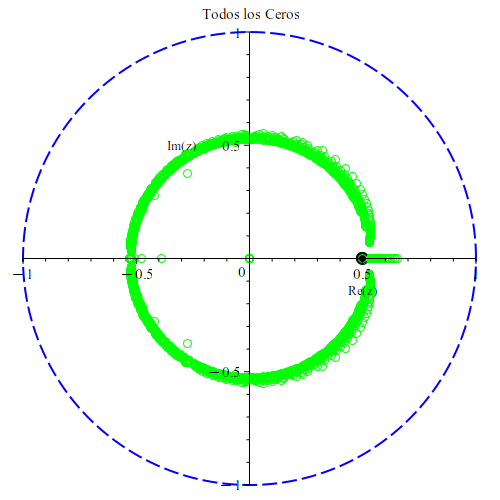
\includegraphics[width=0.46\textwidth]{figures/ceros_interior.png}
		\hfill
		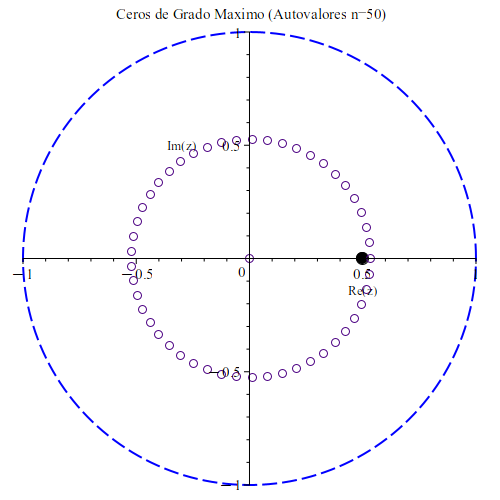
\includegraphics[width=0.46\textwidth]{figures/cero_interior.png}
		\caption{Caso con átomo interior.}
		\label{fig:esqueleto_caso_interior}
	\end{figure}

	\begin{table}[htbp]
		\centering
		\begin{tabular}{c|c|c|c|c}
			$n$  & $\sigma_0^{(n)}$ & $\sigma_1^{(n)}$ & $\sigma_1^{(n)}$ & $\rho_n$ \\
			\hline
			$50$ & $1.5417$         & $1.0000$         & $1.0000$         & $0.5333$
		\end{tabular}
		\caption{Valores singulares relevantes y radio exterior en el caso con átomo interior.}
		\label{tab:esqueleto_caso_interior}
	\end{table}

	% TODO: Añadir aquí un párrafo corto de lectura del ejemplo interior,
	% explicando qué se observa en los ceros y en las ramas singulares.
\end{exm}

\begin{exm}

	Consideramos el producto de Sobolev $\langle p,q\rangle_S=\int_{\mathbb S_1}p(z)\overline{q(z)}\,d\mathbf m_{0;1}(z)+p'(2)\overline{q'(2)}$,
	y fijamos el grado máximo $N=50$. En este caso hay exactamente una rama singular divergente, de modo que la última rama divergente es $\sigma_0^{(n)}$ y la primera rama acotada es $\sigma_1^{(n)}$. El ejemplo debe ilustrar la coexistencia entre esa rama divergente, la primera rama acotada y un cero exterior atraído por el átomo responsable de la inestabilidad.

	\begin{figure}[htbp]
		\centering
		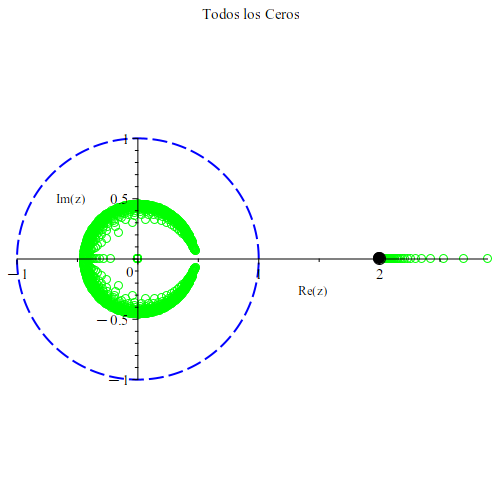
\includegraphics[width=0.46\textwidth]{figures/ceros_exterior.png}
		\hfill
		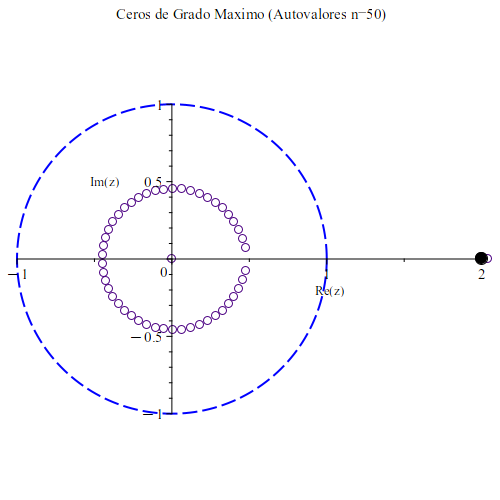
\includegraphics[width=0.46\textwidth]{figures/cero_exterior.png}
		\caption{Caso con un átomo estrictamente exterior.}
		\label{fig:esqueleto_caso_exterior}
	\end{figure}

	\begin{table}[htbp]
		\centering
		\begin{tabular}{c|c|c|c|c|c}
			$n$  & $\sigma_0^{(n)}$       & $\sigma_0^{(n)}$       & $\sigma_1^{(n)}$ & $\sigma_1^{(n)}$ & $\rho_n$ \\
			\hline
			$50$ & $8.9039\times 10^{12}$ & $8.9039\times 10^{12}$ & $1.0000$         & $1.0000$         & $2.0411$
		\end{tabular}
		\caption{Valores singulares relevantes y radio exterior en el caso estrictamente exterior.}
		\label{tab:esqueleto_caso_exterior}
	\end{table}

	% TODO: Añadir aquí un párrafo corto de lectura del ejemplo exterior,
	% conectando ramas divergentes, ramas acotadas y atracción del cero de mayor módulo.
\end{exm}

\begin{exm}

	Consideramos el producto de Sobolev $\langle p,q\rangle_S=\int_{\mathbb S_1}p(z)\overline{q(z)}\,d\mathbf m_{0;1}(z)+p'(0)\overline{q'(0)}+p'(2)\overline{q'(2)}$,
	y fijamos el grado máximo $N=50$. En este ejemplo también hay exactamente una rama singular divergente, de modo que la última rama divergente es $\sigma_0^{(n)}$ y la primera rama acotada es $\sigma_1^{(n)}$. El objetivo es visualizar simultáneamente el desacople entre la geometría exterior y el efecto del átomo interior.

	\begin{figure}[htbp]
		\centering
		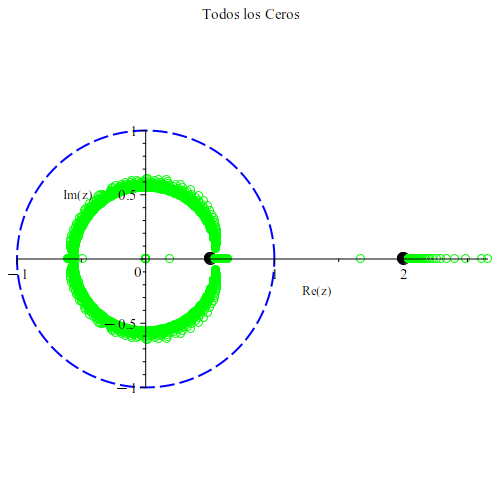
\includegraphics[width=0.46\textwidth]{figures/ceros_mixto.png}
		\hfill
		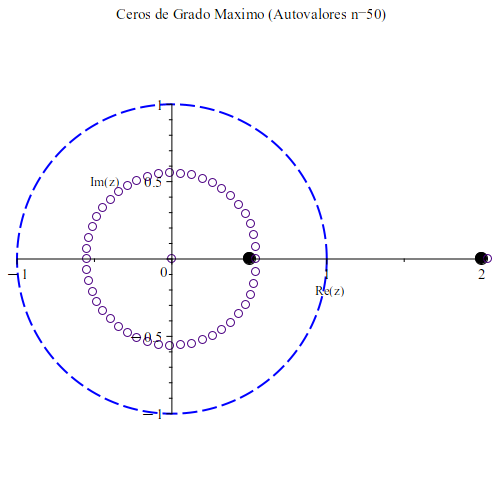
\includegraphics[width=0.46\textwidth]{figures/cero_mixto.png}
		\caption{Caso mixto.}
		\label{fig:esqueleto_caso_mixto}
	\end{figure}

	\begin{table}[htbp]
		\centering
		\begin{tabular}{c|c|c|c|c|c}
			$n$  & $\sigma_0^{(n)}$       & $\sigma_0^{(n)}$       & $\sigma_1^{(n)}$ & $\sigma_2^{(n)}$ & $\rho_n$ \\
			\hline
			$50$ & $8.9038\times 10^{12}$ & $8.9038\times 10^{12}$ & $1.5417$         & $1.0000$         & $2.0411$
		\end{tabular}
		\caption{Valores singulares relevantes y radio exterior en el caso mixto.}
		\label{tab:esqueleto_caso_mixto}
	\end{table}

	% TODO: Añadir aquí un párrafo corto de lectura del ejemplo mixto,
	% subrayando qué se observa en la separación entre ramas divergentes, ramas acotadas y ceros exteriores.
\end{exm}

Como consecuencia colateral del régimen puramente exterior, se recupera también una acotación uniforme global de los ceros. La incluimos solo como corolario de cierre técnico, no como nuevo paso estructural del capítulo.

\begin{thm}\label{thm:acotacion_via_Q_m}
	Sea
	\[
		\langle p,q\rangle_S
		=
		\int_{\mathbb S_R}p(z)\overline{q(z)}\,d\mathbf m_{0;R}(z)
		+
		\sum_{k=1}^m p'(c_k)\overline{q'(c_k)},
	\]
	donde $c_1,\dots,c_m$ son distintos y satisfacen $|c_k|>R$. Sean $\phi_n$ los polinomios ortonormales de Sobolev asociados.
	Entonces existe un compacto $K\subset\mathbb{C}$ tal que todo cero de $\phi_n$, para todo $n\ge 1$, pertenece a $K$.
\end{thm}

\begin{proof}
	Fijemos $\varepsilon>0$ tal que las bolas $\overline{\mathbb{D}_{\varepsilon}(c_k)}$, $1\le k\le m$, sean disjuntas dos a dos.

	Por el Teorema~\ref{thm:atraccion}, existe $n_\varepsilon$ tal que para todo $n\ge n_\varepsilon$ los ceros de $\phi_{n+1}$ con módulo mayor que $R+\varepsilon$ pertenecen al compacto
	\[
		K_\varepsilon:=\overline{\mathbb{D}_{R+\varepsilon}}\cup
		\bigcup_{k=1}^m\overline{\mathbb{D}_{\varepsilon}(c_k)}.
	\]
	Los restantes ceros ya pertenecen a $\overline{\mathbb D_{R+\varepsilon}}$, luego todos los ceros de $\phi_{n+1}$ están en $K_\varepsilon$ para $n\ge n_\varepsilon$.
	Para los grados $1\le n\le n_\varepsilon$, el conjunto total de ceros es finito; sea $K_0$ su envoltura compacta.

	Tomando $K:=K_\varepsilon\cup K_0$ se concluye.
\end{proof}

Queda así cerrada la cadena conceptual del capítulo:
\[
	\begin{aligned}
		Q_k & \longrightarrow \text{umbral singular}                       \\
		    & \longrightarrow \text{Weyl--Horn como techo}                 \\
		    & \longrightarrow \text{reducción racional exterior + Rouché}.
	\end{aligned}
\]
El papel de cada pieza ya queda separado. El Capítulo~\ref{sec:codimension_qk} introdujo los índices $Q_k$, el Capítulo~\ref{sec:estabilizacion} identificó el umbral $m$, el Capítulo~\ref{sec:matricial} lo tradujo a valores singulares, y aquí ese umbral pasó a control de autovalores y finalmente a localización de ceros.

En el régimen puramente exterior $|c_k|>R$ se obtiene primero el conteo exacto y después la atracción hacia los átomos estrictamente exteriores. En el caso mixto sin frontera, el mismo factor racional exterior sigue gobernando la geometría macroscópica, mientras que los átomos interiores solo modifican constantes de estabilización. En la frontera pura $|c_k|=R$, la atracción subsiste pero cambia de escala: ya no se ve a distancia fija del círculo, sino en la capa radial de grosor $1/n$, gobernada por la función
\[
	H(x)=e^x-3\int_0^1 t e^{xt}\,dt
\]
y raíz positiva
\[
	x_*\approx 1.36078.
\]

En el caso mixto con frontera, ambas escalas conviven sin confundirse: macroscópicamente, $F_{\mathrm{out}}$ sigue gobernando el conteo exterior y, por el Corolario~\ref{cor:atraccion_exterior_mixto_frontera}, la atracción hacia los átomos estrictamente exteriores; microscópicamente, cada átomo frontera presenta el mismo perfil $H(x)$, ahora multiplicado por $F_{\mathrm{out}}(c_\ell)$, sin desplazar la raíz positiva límite $x_*$. En consecuencia, en todos los regímenes tratados aquí queda resuelta la localización de ceros. Lo que permanece abierto no es ya el patrón geométrico de esos ceros, sino la determinación exacta de $Q_m(\D)$ en el caso mixto más allá de su mera finitud.
